\documentclass[a4paper, onecolumn]{article}
\usepackage[spanish]{babel}
\usepackage{caption}
\usepackage{graphicx}
\usepackage{amsmath}
\usepackage[utf8]{inputenc}
\usepackage{multirow}
% Configure bibtext
\usepackage{cite}
\setlength{\parindent}{0pt}

\author{Josué Villasante}
\title{Espectroscopía gamma utilizando detectores de NaI, HPGe y BGO en Radess}

\begin{document}
	\maketitle
	\begin{abstract}
		Se presenta los resultados obtenidos luego de realizar espectroscopia gamma para diferentes fuentes radioactivas y diferentes detectores. Además se realizó la calibración en energía y en eficiencia.
	\end{abstract}

	\section{Introducción}
		El objetivo del presente informe es mostrar y comparar los diferentes espectros obtenido de diferentes fuentes y detectores. Las fuentes disponibles fueron ${}^{137}\mathrm{Cs}$, ${}^{22}\mathrm{Na}$ y ${}^{60}\mathrm{Co}$. Los detectores disponibles fueron NaI3x3, HPGe y BGO. Con las detecciones se obtuvo la calibración en energía y en eficiencia, y se identificó una fuente desconocida.
	\section{Materiales y método}
		Se utilizó el simulador Radess. En este no es posible controlar el voltaje de la fuente de alto voltaje, ni la ganancia dada por el amplificador. Por lo tanto, estos no se modificaron. La fuente de alto voltaje se mantuvo constante en 900 voltios. Sin embargo, sí se controló el tiempo de medición y la distancia entre la fuente y el detector.

	\section{Resultados}	
		Se trabajó con los siguientes detectores: NaI3x3, HPGe y BGO. Por cada uno se realizó una calibración utilizando diversos isótopos incluidos en el cuadro \ref{table_energies}.

		\begin{center}
			{\renewcommand{\arraystretch}{1.5}
			\renewcommand{\tabcolsep}{0.2cm}
			\captionof{table}{Isotipos utlizados en la calibración y sus energías de decaimiento gamma. \cite{university_co-60_nodate}\cite{university_cs-137_nodate}\cite{university_na-22_nodate}}
			\label{table_energies}
			\begin{tabular}{ c c c }
				\hline
				Isótopo & Probabilidad(\%) & Energía (keV) \\
				\hline
				${}^{137}\mathrm{Cs}$ & 85 & 662 \\ 
				${}^{22}\mathrm{Na}$ & 180 & 511 \\ 
				${}^{22}\mathrm{Na}$ & 100 & 1275 \\ 
				${}^{60}\mathrm{Co}$ & 99 & 1173 \\ 
				${}^{60}\mathrm{Co}$ & 100 & 1332
			\end{tabular}}
		\end{center}

		Para encontrar el centroide en cada pico se realizó el ajuste a una distribución normal.
		$$
		f(x)=\frac{1}{\sigma \sqrt{2 \pi}} e^{-\frac{1}{2}\left(\frac{x-\mu}{\sigma}\right)^2}
		$$

		\subsection{Calibración en energía}
		Primero se obtuvieron los espectros para el detector de NaI3x3. Para todas las fuentes se configuró una actividad de $10^5$Bq y se realizó la medición por 5 segundos a una distancia de 1cm. La única excepción fue para el ${}^{60}\mathrm{Co}$. Su medición se realizó por 15 segundos.

		\begin{center}
			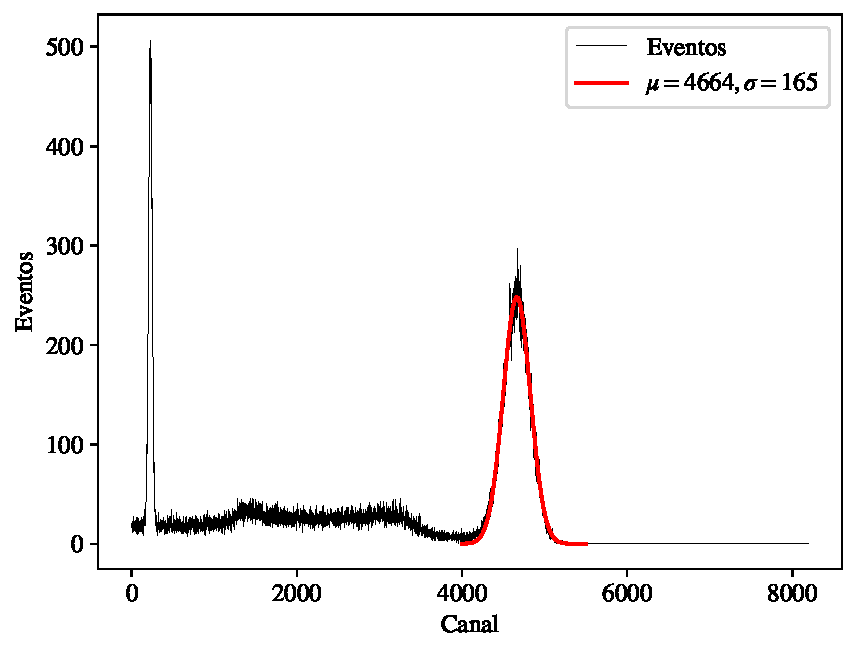
\includegraphics[width=210pt]{img/nai_33_cs_137.pdf}
			\captionof{figure}{Espectro de una fuente de ${}^{137}\mathrm{Cs}$ obtenido de un detector NaI3x3 ajustado a una distribución normal.}
		\end{center}

		\begin{center}
			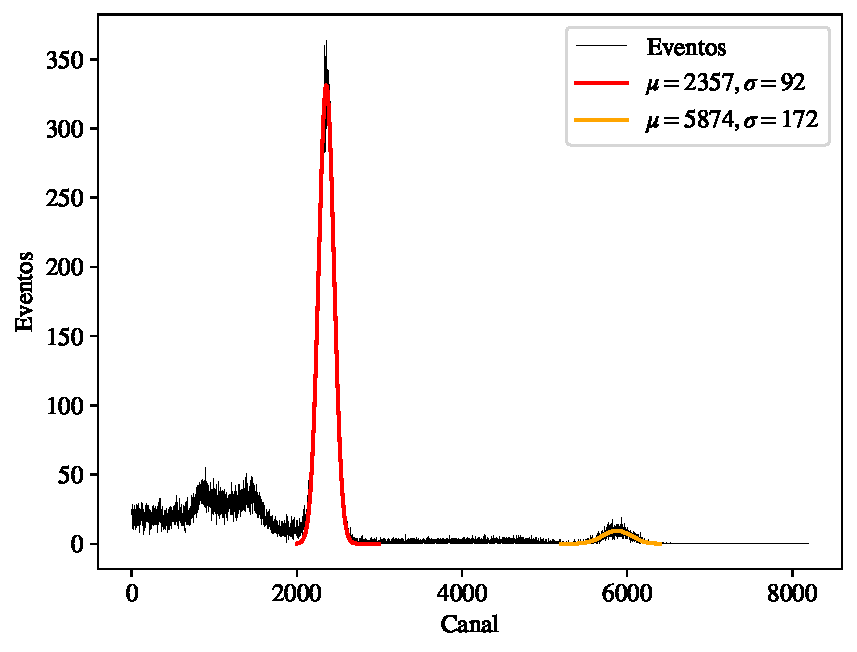
\includegraphics[width=210pt]{img/nai_33_na_22.pdf}
			\captionof{figure}{Espectro de una fuente de ${}^{22}\mathrm{Na}$ obtenido de un detector NaI3x3 ajustado a un par de distribuciones normales.}
		\end{center}

		\begin{center}
			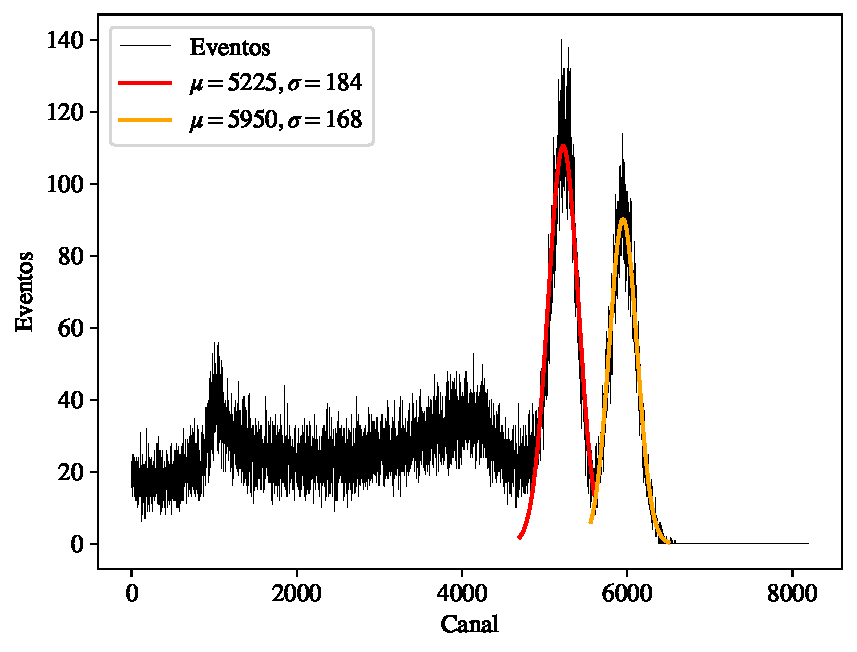
\includegraphics[width=210pt]{img/nai_33_co_60.pdf}
			\captionof{figure}{Espectro de una fuente de ${}^{60}\mathrm{Co}$ obtenido de un detector NaI3x3 ajustado a un par de distribuciones normales.}
		\end{center}

		Con estas mediciones y tomando en cuenta las energías teóricas se realizó la calibración de la energía respecto al canal. En este caso se realizó un ajuste lineal. La energía está dada por

		$$
		E=ax+b
		$$

		donde x es el canal.

		\begin{center}
			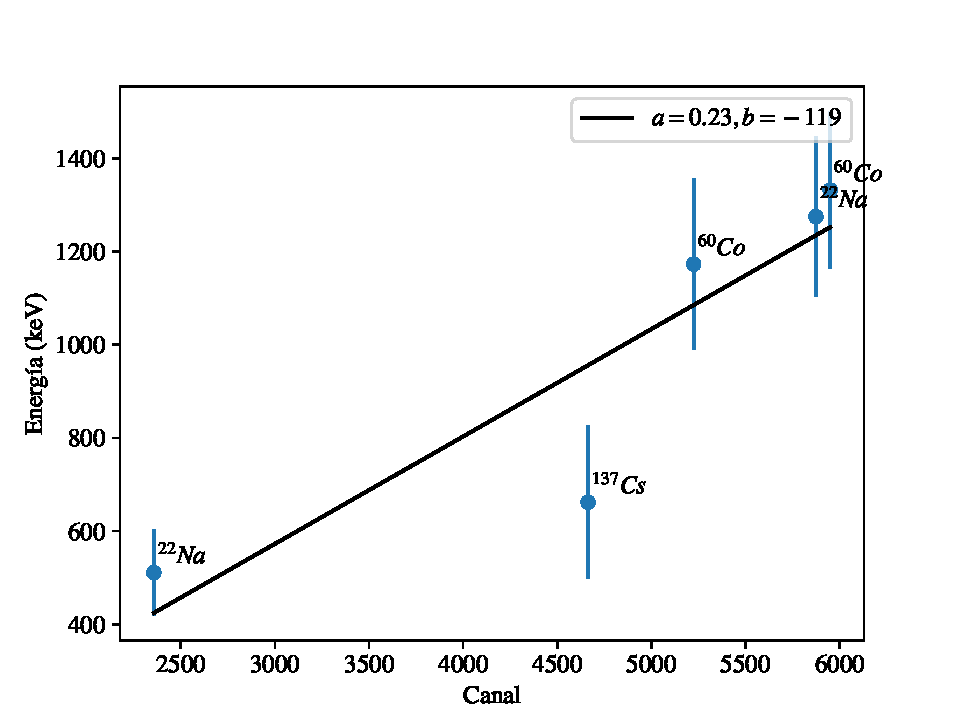
\includegraphics[width=210pt]{img/cal_nai_33.pdf}
			\captionof{figure}{Curva de calibración de la energía respecto al canal para el detector NaI3x3 utilizando fuentes de ${}^{137}\mathrm{Cs}$, ${}^{22}\mathrm{Na}$ y ${}^{60}\mathrm{Co}$.}
		\end{center}

		Con este resultado de pudo comparar la energía dada por la curva de calibración con la energía teórica.

		\begin{center}
			{\renewcommand{\arraystretch}{1.5}
			\renewcommand{\tabcolsep}{0.2cm}
			\captionof{table}{Comparación entre la energía esperada por la curva de calibración y la energía teórica para el detector NaI3x3.}
			\begin{tabular}{ c c c c }
				\hline
				Isótopo & Probabilidad(\%) & Energía teórica (keV) & Energía esperada (keV) \\
				\hline
				${}^{137}\mathrm{Cs}$ & 85 & 662 & 782.29\\ 
				${}^{22}\mathrm{Na}$ & 180 & 511 & 502.76\\ 
				${}^{22}\mathrm{Na}$ & 100 & 1275 & 1314.75 \\ 
				${}^{60}\mathrm{Co}$ & 99 & 1173 & 996.23 \\ 
				${}^{60}\mathrm{Co}$ & 100 & 1332 & 1356.97
			\end{tabular}}
		\end{center}

		Luego se obtuvieron los resultados para el detector HPGe. Igualmente para todos las fuentes se configuró una actividad de $10^5$Bq y se realizó la medición por 30 segundos a una distancia de 1cm.

		\begin{center}
			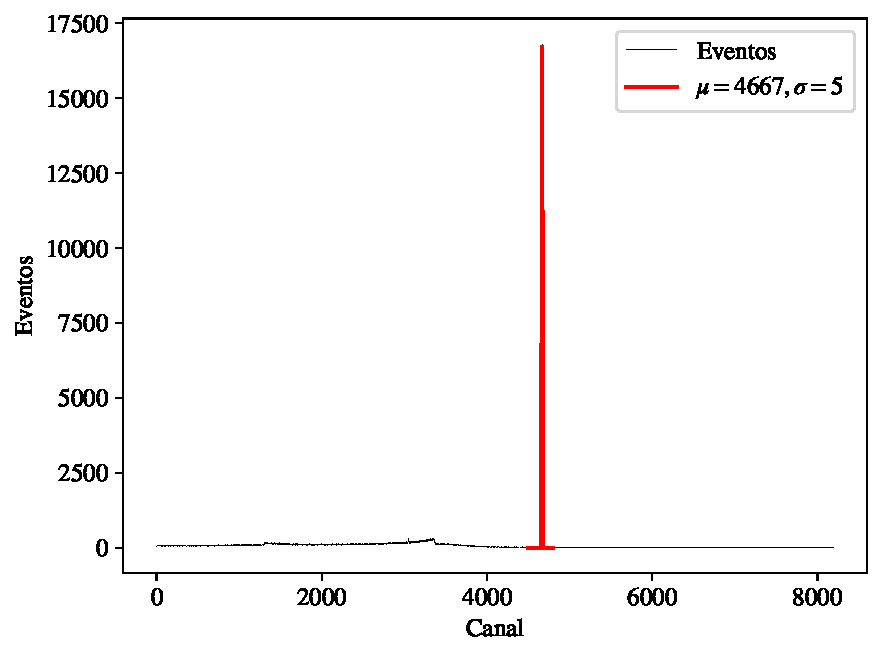
\includegraphics[width=210pt]{img/hpge_cs_137.pdf}
			\captionof{figure}{Espectro de una fuente de ${}^{137}\mathrm{Cs}$ obtenido de un detector HPGe ajustado a una distribución normal.}
		\end{center}

		\begin{center}
			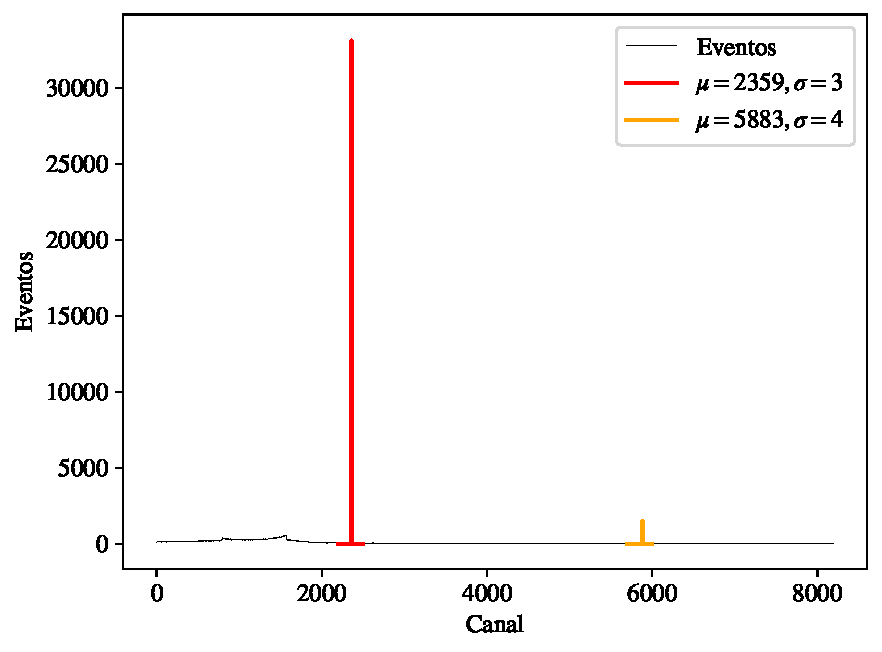
\includegraphics[width=210pt]{img/hpge_na_22.pdf}
			\captionof{figure}{Espectro de una fuente de ${}^{22}\mathrm{Na}$ obtenido de un detector HPGe ajustado a dos distribuciones normales.}
		\end{center}

		\begin{center}
			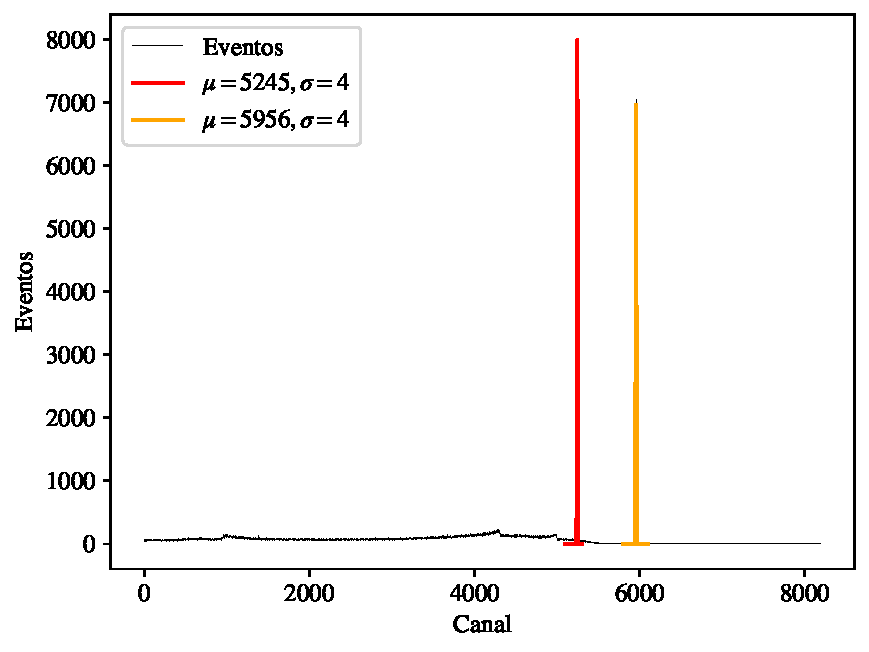
\includegraphics[width=210pt]{img/hpge_co_60.pdf}
			\captionof{figure}{Espectro de una fuente de ${}^{60}\mathrm{Co}$ obtenido de un detector HPGe ajustado a dos distribuciones normales.}
		\end{center}

		Igualmente se realizó la calibración de la energía respecto al canal.

		\begin{center}
			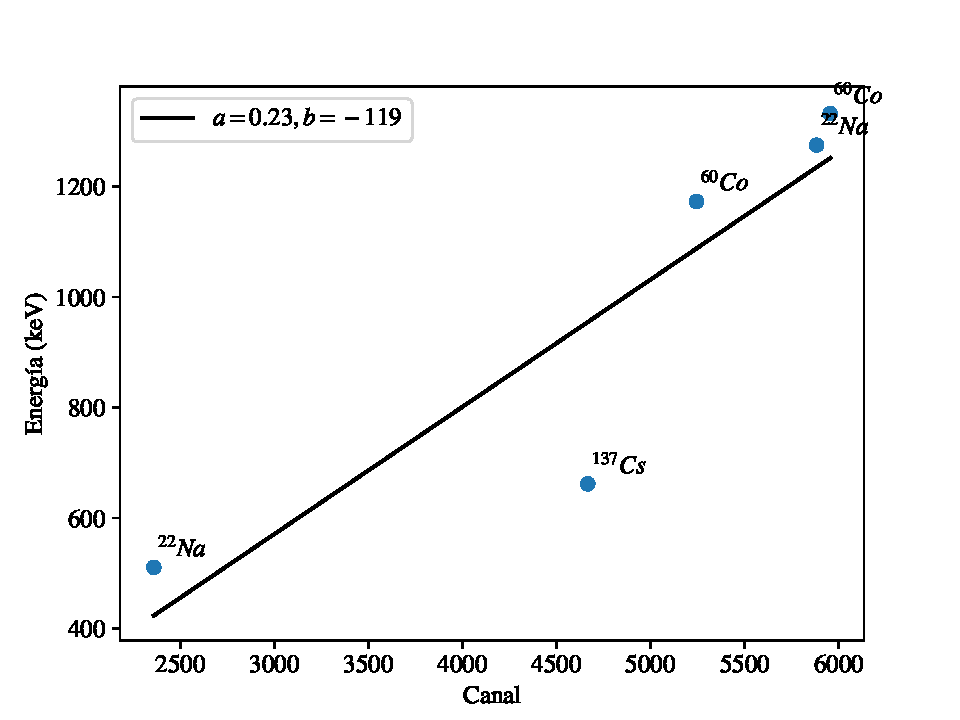
\includegraphics[width=210pt]{img/cal_hpge.pdf}
			\captionof{figure}{Curva de calibración de la energía respecto al canal para el detector HPGe utilizando fuentes de ${}^{137}\mathrm{Cs}$, ${}^{22}\mathrm{Na}$ y ${}^{60}\mathrm{Co}$.}
		\end{center}

		Con este resultado de pudo comparar la energía dada por la curva de calibración con la energía teórica.

		\begin{center}
			{\renewcommand{\arraystretch}{1.5}
			\renewcommand{\tabcolsep}{0.2cm}
			\captionof{table}{Comparación entre la energía esperada por la curva de calibración y la energía teórica para el detector HPGe.}
			\begin{tabular}{ c c c c }
				\hline
				Isótopo & Probabilidad(\%) & Energía teórica (keV) & Energía esperada (keV) \\
				\hline
				${}^{137}\mathrm{Cs}$ & 85 & 662 & 777.96\\ 
				${}^{22}\mathrm{Na}$ & 180 & 511 & 502.86\\ 
				${}^{22}\mathrm{Na}$ & 100 & 1275 & 1315.91 \\ 
				${}^{60}\mathrm{Co}$ & 99 & 1173 & 999.76 \\ 
				${}^{60}\mathrm{Co}$ & 100 & 1332 & 1356.50
			\end{tabular}}
		\end{center}

		Finalmente se obtuvieron los resultados para el detector BGO. De igual manera, para todos las fuentes se configuró una actividad de $10^5$Bq y se realizó la medición por 5 segundos a una distancia de 1cm. La única excepción fue para el ${}^{60}\mathrm{Co}$. Su medición se realizó por 10 segundos.

		\begin{center}
			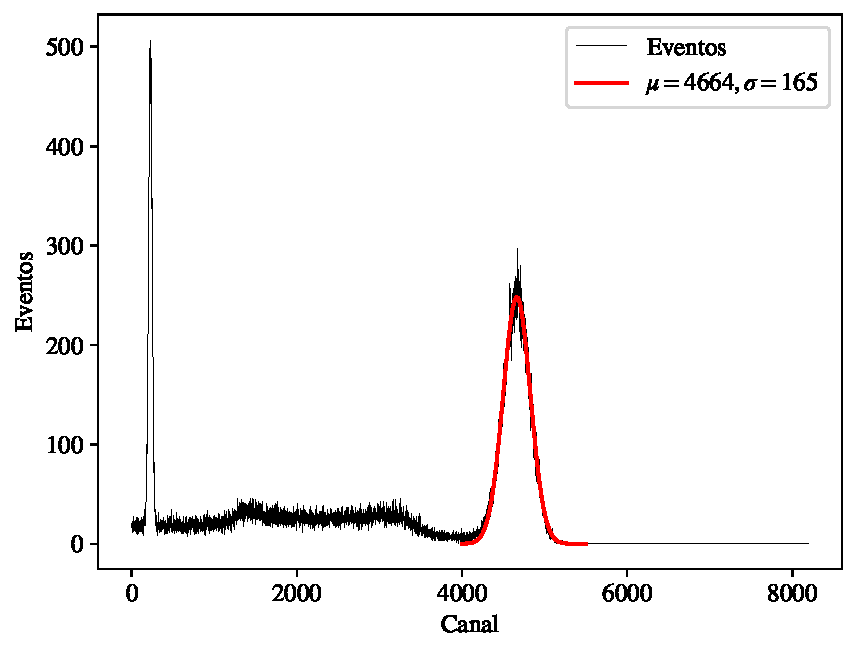
\includegraphics[width=210pt]{img/nai_33_cs_137.pdf}
			\captionof{figure}{Espectro de una fuente de ${}^{137}\mathrm{Cs}$ obtenido de un detector BGO ajustado a una distribución normal.}
		\end{center}

		\begin{center}
			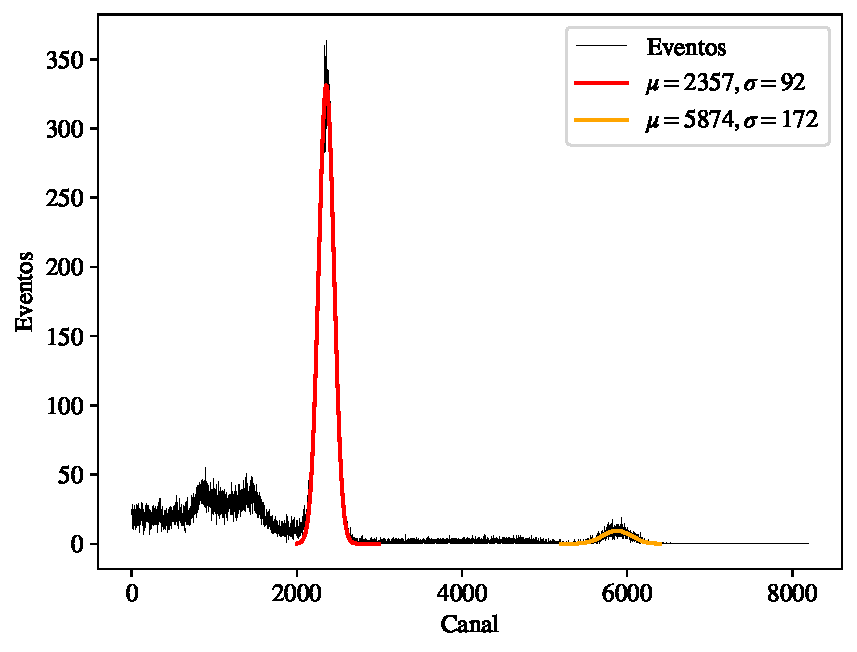
\includegraphics[width=210pt]{img/nai_33_na_22.pdf}
			\captionof{figure}{Espectro de una fuente de ${}^{22}\mathrm{Na}$ obtenido de un detector BGO ajustado a un par de distribuciones normales.}
		\end{center}

		\begin{center}
			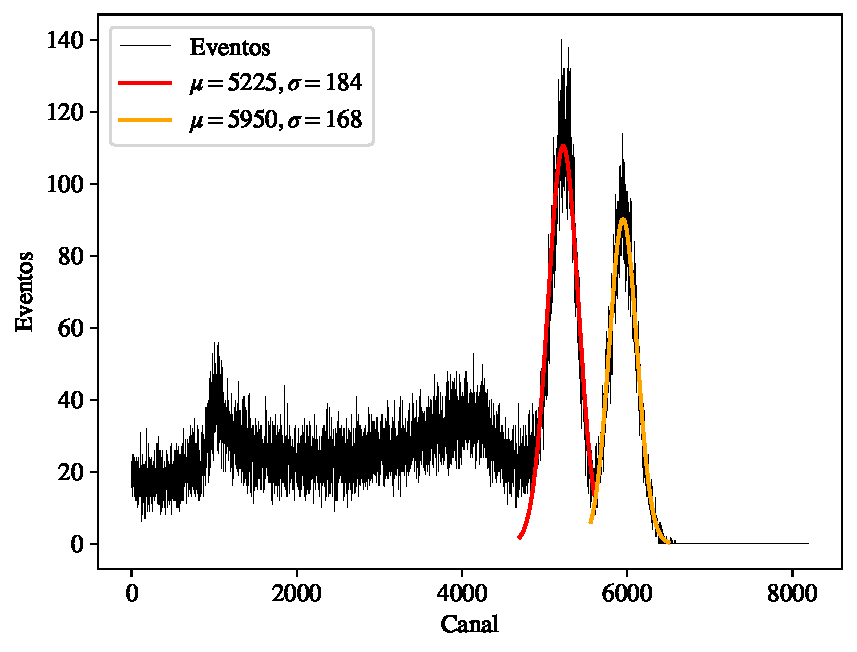
\includegraphics[width=210pt]{img/nai_33_co_60.pdf}
			\captionof{figure}{Espectro de una fuente de ${}^{60}\mathrm{Co}$ obtenido de un detector BGO ajustado a un par de distribuciones normales.}
		\end{center}

		Igualmente se realizó la calibración de la energía respecto al canal.

		\begin{center}
			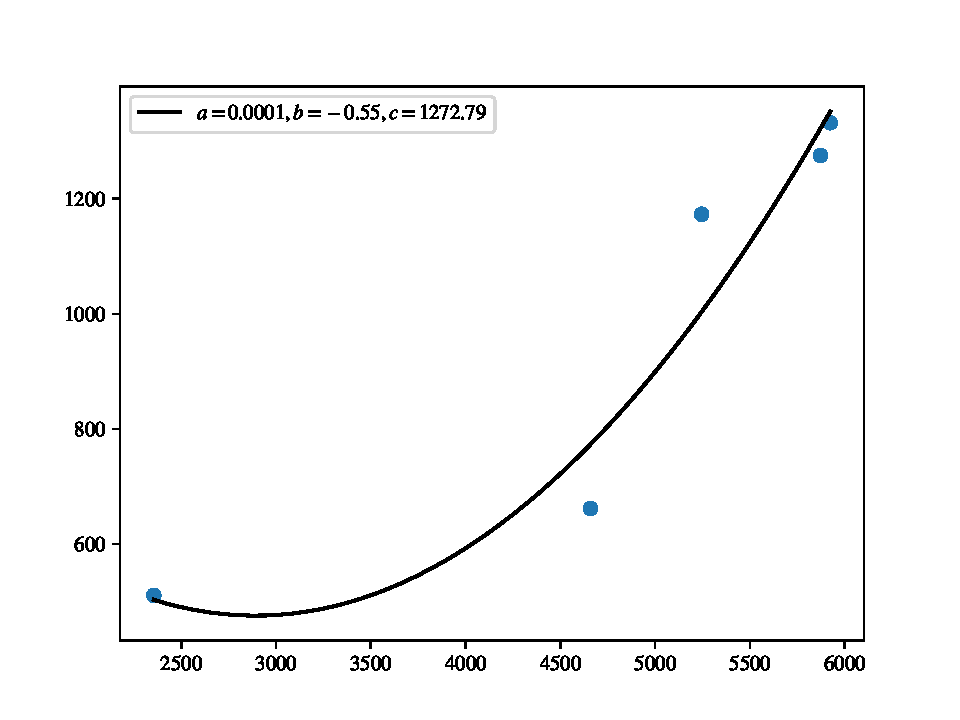
\includegraphics[width=210pt]{img/cal_bgo.pdf}
			\captionof{figure}{Curva de calibración de la energía respecto al canal para el detector BGO utilizando fuentes de ${}^{137}\mathrm{Cs}$, ${}^{22}\mathrm{Na}$ y ${}^{60}\mathrm{Co}$.}
		\end{center}

		Con este resultado de pudo comparar la energía dada por la curva de calibración con la energía teórica.

		\begin{center}
			{\renewcommand{\arraystretch}{1.5}
			\renewcommand{\tabcolsep}{0.2cm}
			\captionof{table}{Comparación entre la energía esperada por la curva de calibración y la energía teórica para el detector BGO.}
			\label{table_expected_energies}
			\begin{tabular}{ c c c c }
				\hline
				Isótopo & Probabilidad(\%) & Energía teórica (keV) & Energía esperada (keV) \\
				\hline
				${}^{137}\mathrm{Cs}$ & 85 & 662 & 773.11\\ 
				${}^{22}\mathrm{Na}$ & 180 & 511 & 503.15\\ 
				${}^{22}\mathrm{Na}$ & 100 & 1275 & 1321.91 \\ 
				${}^{60}\mathrm{Co}$ & 99 & 1173 & 1003.48 \\ 
				${}^{60}\mathrm{Co}$ & 100 & 1332 & 1351.35
			\end{tabular}}
		\end{center}

		\subsection{Calibración en eficiencia}

		La calibración en eficiencia se realizó para los tres detectores. Para esto se tomó en cuenta que la eficiencia está definida por
		$$
		E = \frac{N}{AYt}
		$$
		donde $E$ es eficiencia, $N$ es el número de cuentas, $A$ es la actividad de la fuente, $Y$ es la probabilidad de desintegración y $t$ es el tiempo de medición. Para el número de cuentas se tomó aquellas dentro de {\it full width at height maximum} (FWHM). Es decir, donde el canal es igual a $\mu\pm2.355\sigma$. Como ya se había mencionado antes, $A=10^5$. Los tiempos de medición también ya se mencionaron anteriormente para cada caso, y la probabilidad de desintegración se encuentra en el cuadro \ref{table_expected_energies}.

		Para el ajuste se tomó en cuenta una función del tipo

		$$
		E = ax^3 + bx^2 + cx + d
		$$

		\begin{center}
			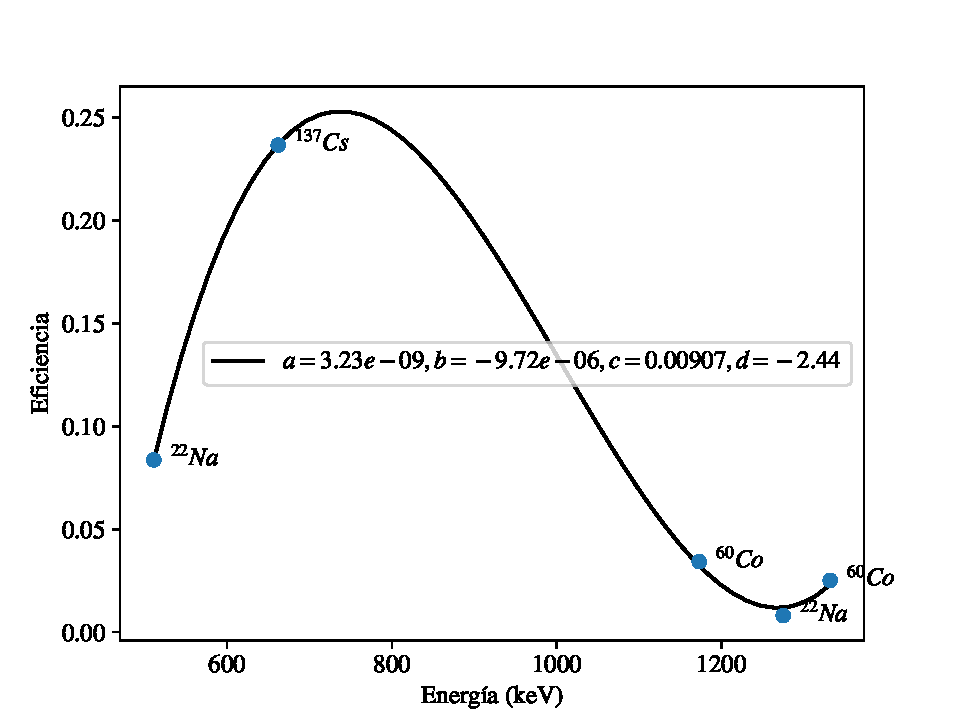
\includegraphics[width=210pt]{img/nai_33_efficiency.pdf}
			\captionof{figure}{Eficiencia para cada pico de energía dado por el detector NaI3x3 y su ajuste a una curva.}
		\end{center}


		\begin{center}
			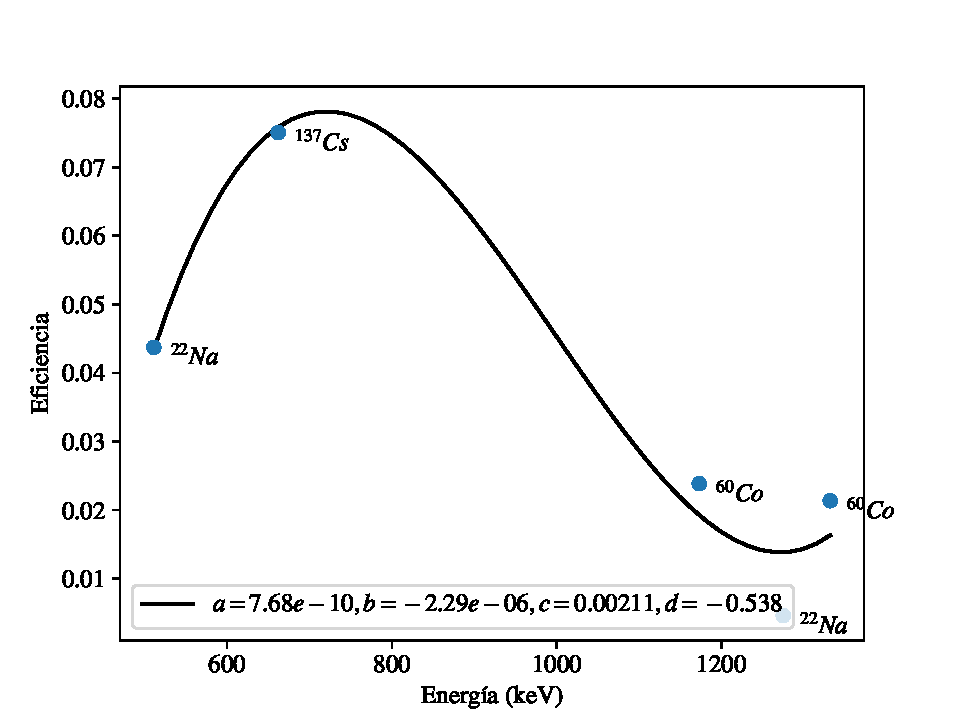
\includegraphics[width=210pt]{img/hpge_efficiency.pdf}
			\captionof{figure}{Eficiencia para cada pico de energía dado por el detector HPGe y su ajuste a una curva.}
		\end{center}

		\begin{center}
			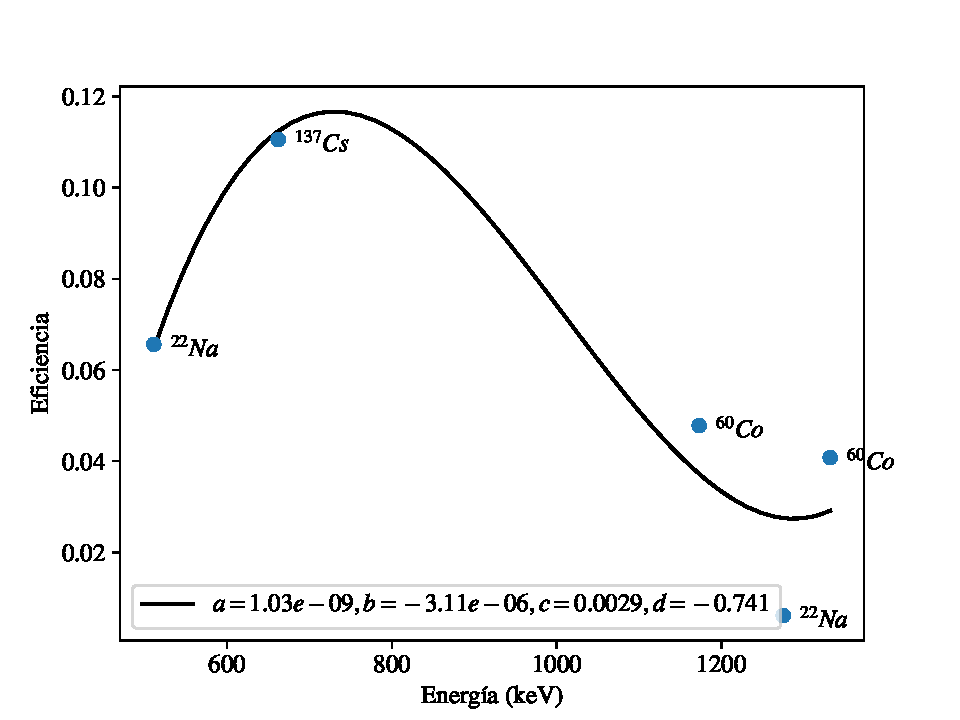
\includegraphics[width=210pt]{img/bgo_efficiency.pdf}
			\captionof{figure}{Eficiencia para cada pico de energía dado por el detector BGO y su ajuste a una curva.}
		\end{center}

		\subsection{Resolución de energía}

		Según Knoll \cite{knoll_radiation_2010}, la energía guarda la siguiente relación con la resolución.
		$$
		R \equiv \frac{\mathrm{FWHM}}{H_0}
		$$

		Como hemos hecho un ajuste gaussiano, podemos obtener la resolución para cada pico utilizando
		$$
		R = \frac{2.355\sigma}{\mu}
		$$

		\begin{center}
			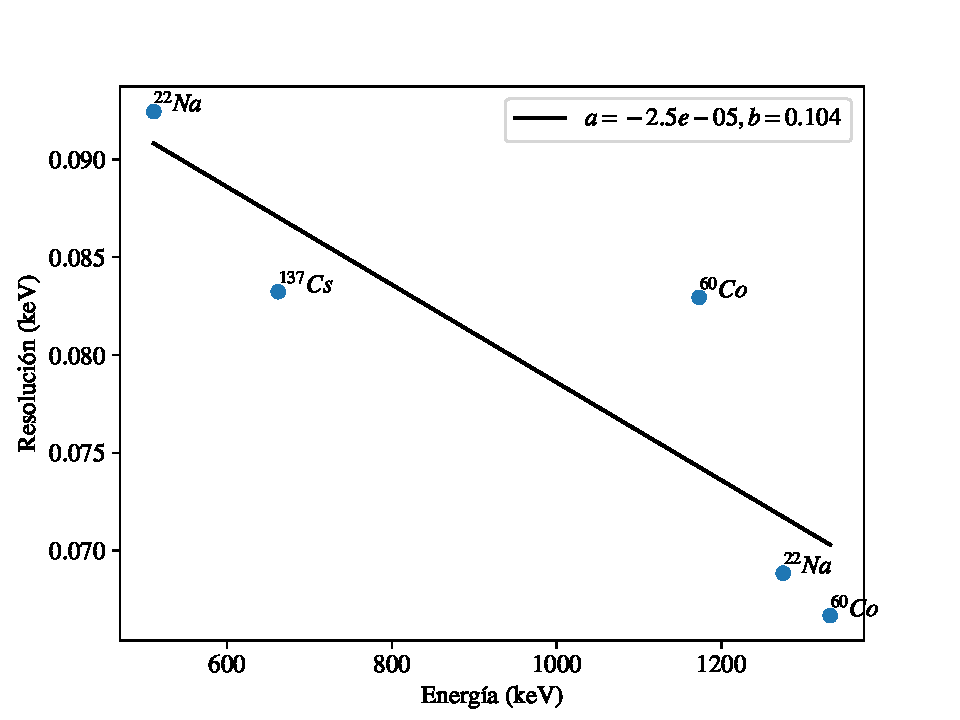
\includegraphics[width=210pt]{img/resolution_vs_energy.pdf}
			\captionof{figure}{Resolución versus energía para los picos obtenidos del detector NaI3x3.}
		\end{center}

		\begin{center}
			{\renewcommand{\arraystretch}{1.5}
			\renewcommand{\tabcolsep}{0.2cm}
			\captionof{table}{Resolución de energía para cada pico obtenido del detector NaI3x3.}
			\label{table_energy_resolution}
			\begin{tabular}{ c c c  }
				\hline
				Isótopo & Energía teórica (keV) & Resolución (keV) \\
				\hline
				${}^{137}\mathrm{Cs}$ & 662 & 0.0832\\ 
				${}^{22}\mathrm{Na}$  & 511 & 0.0924\\ 
				${}^{22}\mathrm{Na}$  & 1275 & 0.0688 \\ 
				${}^{60}\mathrm{Co}$ & 1173 & 0.0829 \\ 
				${}^{60}\mathrm{Co}$  & 1332 & 0.0666
			\end{tabular}}
		\end{center}

		\subsection{Identificación de una fuente desconocida}
		Utilizando el detector NaI3x3 y la calibración antes obtenida, se obtuvo la espectroscopía de una fuente desconocida y se pudo identificar los pico de energía.
		\begin{center}
			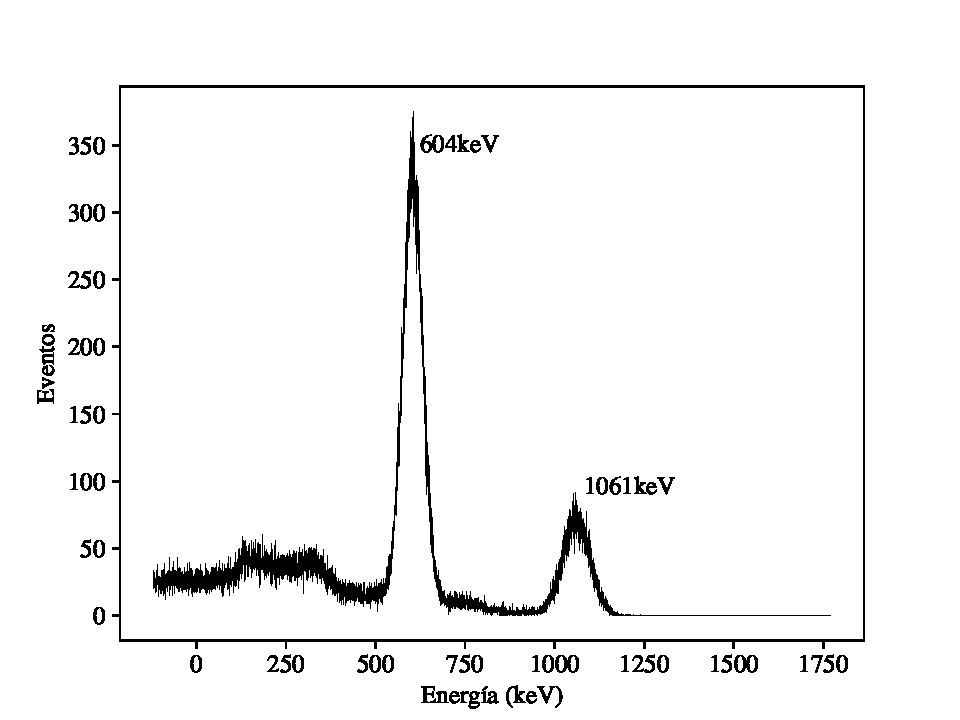
\includegraphics[width=210pt]{img/unknown_source.pdf}
			\captionof{figure}{Espectroscopía de una fuente desconocida.}
		\end{center}
		\begin{center}
			{\renewcommand{\arraystretch}{1.5}
			\renewcommand{\tabcolsep}{0.2cm}
			\captionof{table}{Identificación de posibles radionúcleos. \cite{noauthor_eml_1997}}
			\label{table_energy_resolution}
			\begin{tabular}{ c c c c }
				\hline
				& \multicolumn{2}{c}{Posibles núcleos} \\
				\hline
				Energía medida (keV) & Energía (keV) & \% & Núcleo \\
				\hline
				604 & 569 / 511 & 97.8 / 2.9 & \multirow{2}{*}{${}^{207}\mathrm{Bi}$ / ${}^{65}\mathrm{Zn}$}  \\
				1061 & 1063.1 / 1115.5 & 74.9 / 50.8 &  \\
				\hline
			\end{tabular}}
		\end{center}
	\section{Conclusiones}
		Lo primero a notar es la diferencia en resolución entre los detectores. El que produjo mayor error fue el detector BGO, produciendo los mayores valores de $\sigma$ al realizar el ajuste. En cambio el detector HGPe tuvo una muy alta resolución. Al realizar el ajuste prácticamente se obtuvo una delta de Dirac, y un sigma muy pequeño.

		Luego, también notamos la diferencia en eficiencia. Vemos que el detector HPGe es el que obtuvo los menores valores de eficiencia. Por otro lado, el rango de eficiencia del detector NaI3x3 incluye a la eficiencia del detector BGO, por lo que dependiendo de la energía el detector BGO puede ser más o menos eficiente que el detector de NaI3x3.

		Sobre la resolución de energía, vemos que a medida aumenta la energía es mejor la resolución. Por tal motivo, para radio núcleos de mayor energía se obtendrá un resultado más preciso.

		Finalmente, se demostró que cada uno de los picos se pudo ajustar a una distribución normal.
	\bibliography{citations}
	\bibliographystyle{ieeetr}
\end{document}